% Capstone report body, IEEE two-column (IEEEtran conference, A4), as the 2025 winners submitted theirs; the department
% cover is cover.tex. build.sh compiles both and merges them into report.pdf. Abstract: abstract.tex (shared with the cover).
% Sources of every number: SOURCES.md. \member{...} = filled in by the team.
% Figures: column figures are drawn at the column width (8.86 cm); page-wide figures (figure*) are placed at the width they
% were drawn at (14.66 cm), never scaled.
\documentclass[conference,a4paper]{IEEEtran}
\usepackage{fontspec}
\usepackage{xeCJK}
\setmainfont{Liberation Serif}
\setCJKmainfont{Noto Serif TC}
\usepackage{graphicx}
\usepackage{booktabs}
\usepackage{adjustbox}
\usepackage{array}
\usepackage{tabularx}
\usepackage{xcolor}
\usepackage{enumitem}
\usepackage{amsmath}
\usepackage{placeins}
\renewcommand{\topfraction}{0.9}
\renewcommand{\bottomfraction}{0.6}
\renewcommand{\textfraction}{0.1}
\renewcommand{\floatpagefraction}{0.75}
\renewcommand{\dbltopfraction}{0.9}
\renewcommand{\dblfloatpagefraction}{0.75}
\setcounter{topnumber}{3}
\setcounter{dbltopnumber}{2}
\setcounter{totalnumber}{4}
\usepackage[hidelinks]{hyperref}
\setlist{nosep,leftmargin=1.2em}
\newcommand{\pending}[1]{\textcolor{red}{[#1]}}
\newcommand{\member}[1]{\textcolor{blue}{[#1]}}
\pagestyle{plain}

\begin{document}
\title{Beautified Is Not Forged: A Face Checker That Separates Beautification from Forgery and Shows Checkable Evidence}
\author{\IEEEauthorblockN{Qin-Ying Lin, Bo-Rong Chen, Chen-Shan Yu}
\IEEEauthorblockA{National Tsing Hua University, Hsinchu, Taiwan}}
\maketitle
\pagestyle{plain}

\begin{abstract}
% Abstract, shared by cover.tex and report.tex.
Face-forgery detectors answer ``real'' or ``fake''. A genuine photograph that has only been through a beauty app or a
retouching service is neither, and once the skin is smoothed the detectors tend to call it fake. On pixel-aligned pairs of
genuine faces and their commercially smoothed renders, sixteen of seventeen published detectors score the smoothed face as more
forged than its own original. A controlled training experiment shows that the cause is which class saw skin smoothing during
training: showing it to both classes lowers the accusation from 54 to 12 percent. We build on that recipe a face checker that
answers real, forged or beautified, marks the face part its evidence came from, and shows only sentences that code composes from
the model's output and checks before display. Restoring the marked region to its original pixels removes 94 percent of the
model's part-level forgery decisions, about twice what a post-hoc heat map achieves, and free-form descriptions written by
vision-language models fail a blind matching test, so no model is allowed to describe the image. The checker runs in a web
browser and the photograph never leaves the device.

\end{abstract}


% ------------------------------------------------------------------ 1
\section{Motivation and Purpose}

Many face photographs pass through a beauty app or a retouching service before anyone else sees them. Face-forgery detectors,
which are used for content moderation, remote identity checks and fact-checking, answer only ``real'' or ``fake''. A smoothed
genuine face is neither, and the detectors have to put it somewhere.

Figure~\ref{fig:teaser} shows what happens. In panel (a), a genuine FFHQ photograph~\cite{ffhq} is processed by a commercial
retouching service's strongest skin smoothing. Four recent detectors move from ``genuine'' to ``forged'', each at its own
threshold. In panel (b), a face-swap video from Celeb-DF-B~\cite{libourel2024} is passed through an app beauty preset, and
three of the same four detectors now let it through. One edit causes both errors: the smoothed genuine face is accused, and the
beautified forgery escapes.

\begin{figure}[!htb]
\centering
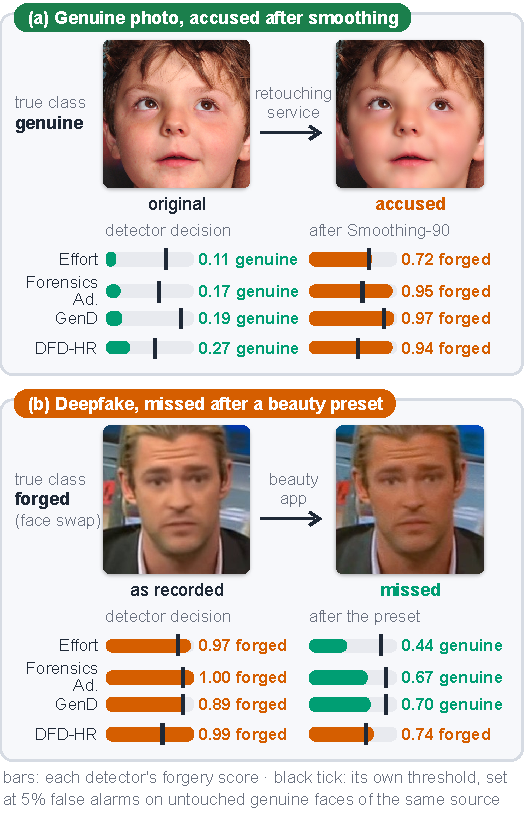
\includegraphics[width=\columnwidth]{figs/fig_teaser.pdf}
\caption{The two errors on real data. (a) A genuine photograph and its commercial Smoothing-90 render
(RetouchingFFHQ~\cite{retouchingffhq}). (b) A Celeb-DF face swap before and after an app beauty preset
(Celeb-DF-B~\cite{libourel2024}). Bars: each detector's forgery score; ticks: its threshold at 5\% false alarms on untouched
genuine faces of the same source.}
\label{fig:teaser}
\end{figure}

Three things are missing from the usual answer. A binary detector has no ``beautified'' output. The usual answer to ``where is
the evidence'' is a post-hoc heat map, and restoring the region such a map marks removes only about half of the decisions it
is supposed to explain (Section~\ref{sec:res-evidence}). The usual answer to ``why'' is a vision-language model describing the
image, and such descriptions are matched to their own photograph about as often as a coin flip (Section~\ref{sec:res-text}).

The purpose of this project is a system that, given one face photograph and no original to compare with, (i) answers real,
forged or beautified, (ii) marks the face part its evidence came from, and (iii) shows only sentences that code can match to
the model's output, while (iv) running on the user's device so that the photograph is not uploaded. Each of the four promises
comes with a test that could fail, and the report states where it does.

% ------------------------------------------------------------------ 2
\section{Related Work and Comparison}
\label{sec:related}

\textbf{Forgery detectors.} Published detectors are trained on FaceForensics++~\cite{ffpp} or on synthetic blends such as
self-blended images~\cite{sbi}, and recent ones adapt CLIP~\cite{clip}: Effort~\cite{effort}, Forensics Adapter~\cite{forensicsadapter},
GenD~\cite{gend2026} and DFD-HR~\cite{dfdhr2026}. All of them output one forgery score. DeepfakeBench~\cite{deepfakebench}
provides released weights for ten CNN detectors, which we use unchanged.

\textbf{Beautification and detectors.} Libourel et al.~\cite{libourel2024} released Celeb-DF-B and measured an AUC drop of
three detectors under app presets. Saeed et al.~\cite{saeed2025} measured beautified forgeries escaping detection. Concas et
al.~\cite{concas2025} applied one smoothing filter and reported both directions for two CNNs. None of them separated the two
directions on pixel-aligned pairs or traced the error to training.

\textbf{Retouching detection.} RetouchingFFHQ~\cite{retouchingffhq} and earlier work~\cite{bharati2016,jain2018} label
retouching operations on genuine photographs but have no forgery class, so they cannot say whether a retouched face is also
forged. Differential detection with a trusted reference~\cite{rathgeb2020diff} needs a second photograph of the same person.

\textbf{Explanations.} Grad-CAM~\cite{gradcam}, Grad-CAM++~\cite{gradcampp} and Score-CAM~\cite{scorecam} are computed after
the fact and are not trained to mark the edited region. FakeVLM~\cite{fakevlm2025} decides and explains in free text.

Table~\ref{tab:compare} summarises the comparison. The project does not claim a better forgery detector; it claims an answer,
a region and sentences that can each be tested.

\begin{table}[!htb]
\centering
\caption{What each line of work provides. ``Tested'' means a test that could fail was run on held-out data.}
\label{tab:compare}
\footnotesize
\setlength{\tabcolsep}{3pt}
\begin{tabular}{@{}lcccc@{}}
\toprule
 & beautified & region & text & on \\
 & answer & tested & checked & device \\
\midrule
Binary detectors~\cite{effort,forensicsadapter,sbi} & no & no & no & some \\
Retouching detectors~\cite{retouchingffhq} & yes\textsuperscript{a} & no & no & -- \\
Post-hoc heat maps~\cite{gradcam,scorecam} & no & weak\textsuperscript{b} & no & yes \\
VLM explainers~\cite{fakevlm2025} & partly & no & no\textsuperscript{c} & no\textsuperscript{d} \\
This project & yes & yes & yes & yes \\
\bottomrule
\end{tabular}\\[2pt]
\parbox{\columnwidth}{\scriptsize \textsuperscript{a}no forgery class; \textsuperscript{b}Table~\ref{tab:restore};
\textsuperscript{c}Table~\ref{tab:vlm}; \textsuperscript{d}18 GB GPU.}
\end{table}

% ------------------------------------------------------------------ 3
\section{Design Principles}

\textbf{Classes are defined by what was changed, not by the tool.} A face is \emph{forged} when the person, expression or
action shown was not captured: an identity swap, a reenactment, a synthesised face or a replaced face part. It is
\emph{beautified} when, after capture, only colour, skin tone, skin texture or the shape of the person's own features changed.
A beautified forgery is forged. This removes the ambiguity of tools that use neural networks for beautification.

\textbf{Every displayed claim has a test.} The answer is tested by a controlled training comparison, the marked region by
restoring it to the original pixels, and every sentence by a rule checker that matches it to the model's output.

\textbf{Measure before claiming.} Each experiment's pass bar was written down before it was run, intervals are computed by
bootstrap over pairs, videos or identities, and failed predictions are reported as failed.

\textbf{Nothing leaves the device.} Face detection, the model, part naming and sentence composition all run in the browser.

% ------------------------------------------------------------------ 4
\section{Methods and Steps}

Figure~\ref{fig:method} gives the method in one figure: three sources of supervision, each with an exact footprint, one
backbone with its heads, the main model's outputs on two held-out images, the three tests that could fail, and the browser.
The next subsections give the measurement protocol, the controlled experiment that finds the cause of the accusation, the
split of commercial renders into single operations, the training recipe, the evidence head and the sentence rules.

\begin{figure*}[t]
\centering
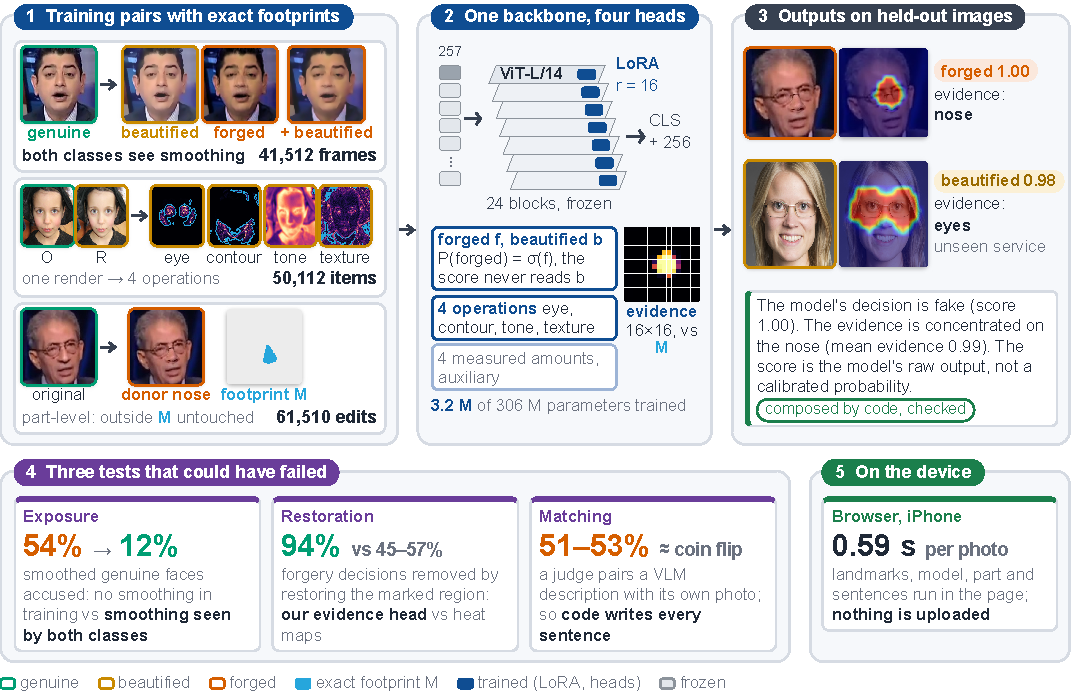
\includegraphics[width=\textwidth]{figs/fig_overview.pdf}
\caption{The method. (1) Training pairs whose footprint $M$ is exact because every edited image has a pixel-aligned original:
an FF++ triplet drawn per step (the forged item is beautified too, half of the time, so both classes see smoothing), a
commercial render split into four single operations (Figure~\ref{fig:engine}), and a part-level forgery. (2) The backbone and
its heads (Figure~\ref{fig:model}); the classifier does not read the evidence map. (3) The main model (seed 1) on a held-out
FF++ forgery with a donor nose and on an Alibaba eye-enlargement render, a service never used in training, with the part its
evidence names and the sentence code composes. (4) The three tests of Sections~\ref{sec:res-cause}, \ref{sec:res-evidence}
and \ref{sec:res-text}. (5) The browser chain of Section~\ref{sec:system}.}
\label{fig:method}
\end{figure*}


\subsection{Measuring the problem in both directions}
\label{sec:protocol}

\emph{Direction A, the accusation.} The test set is 2,210 FFHQ originals and their renders by the Alibaba retouching service
(RetouchingFFHQ), aligned pixel for pixel, so the only difference inside a pair is the retouching. The threshold-free reading
asks in what share of pairs the render scores as more forged than its own original (50\% means no effect). The thresholded
reading fixes, per detector, the threshold that accuses 5\% of the untouched originals and counts the renders above it.

\emph{Direction B, the escape.} Celeb-DF-B holds 232 genuine and 232 deepfake videos, each untreated, beautified by one of four
app presets, and re-encoded without a filter. The effect of beautification alone is the rise in the miss rate under the preset
minus the rise under re-encoding.

Seventeen published detectors are scored with their released weights under each one's own preprocessing; intervals come from
2,000 bootstrap draws over pairs or videos.

\subsection{Finding the cause}
\label{sec:cause}

To find what decides the accusation, one CLIP model is trained on FF++ data only, with one recipe, in arms that differ only in
which class receives skin-smoothed training views (Figure~\ref{fig:exposure}): P0 neither, P3 forged faces only, P1 genuine
faces only, P2 both. No image of any retouching service is used in these arms. The edge treatment of the smoothing is then
varied with its strength held fixed (face-local, whole crop, a ring at the hull edge) to find what the detectors react to.

\begin{figure}[!htb]
\centering
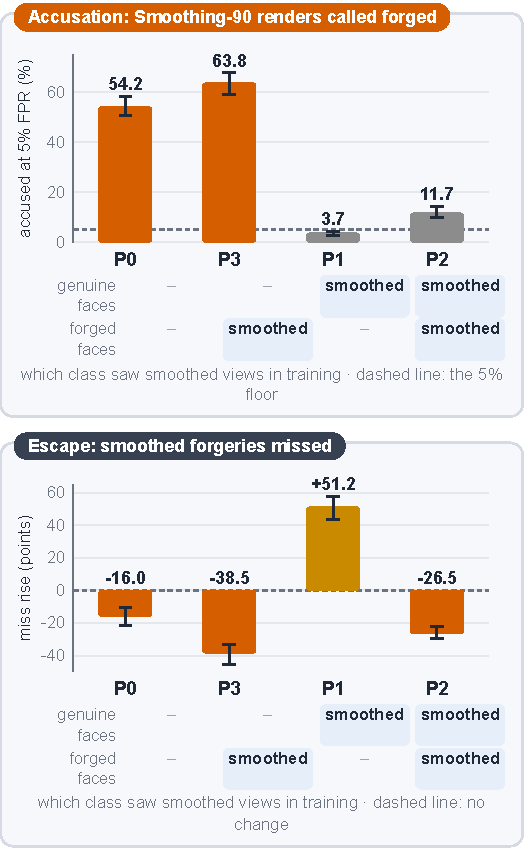
\includegraphics[width=\columnwidth]{figs/fig_exposure.pdf}
\caption{The training-exposure experiment (seed 1, 95\% bootstrap intervals). Under each arm: which class saw skin-smoothed
views in training. Top: commercial Smoothing-90 renders accused at 5\% false alarms on their originals (dashed line: the 5\% floor). Bottom: change in the
miss rate on strongly smoothed Celeb-DF-v2 forgeries (dashed line: no change). Smoothing seen only by forged faces (P3) produces the accusation; seen
only by genuine faces (P1) it produces the escape; seen by both (P2) neither.}
\label{fig:exposure}
\end{figure}

\subsection{Splitting commercial renders into single operations}
\label{sec:engine}

A commercial render applies several operations at once, and the service does not say which or where. Trained on whole
renders, a detector can learn the service instead of the operation, and the footprint of a whole render covers most of the
face, so it says little about where an edit is. Before this step, every footprint in the project came from its own scripted
filters, each with a single parameter.

Figure~\ref{fig:engine} shows the split on one Tencent pair. At 512 pixels, DIS optical flow~\cite{dis} on locally
normalised luminance, which the render's change of tone does not disturb, gives a field $f$ with $O(x+f)\approx R(x)$ and
the inverse field $g$. A mask $m_e$ around the eyes, built from landmarks, splits the geometry: the eye component is
$O(x+m_e f)$ and the contour component $O(x+(1-m_e)f)$. What the warp cannot explain is the residual $P=R-O(x+f)$; a
Gaussian low-pass with $\sigma=6$ pixels gives its tone part and the remainder its texture part, each carried back to the
original's geometry by $g$ and added to $O$. By construction $O(x+f)+P=R$, and the reconstruction measures 108~dB.

Each component is a real piece of a commercial edit, aligned with $O$ pixel for pixel, so it has an exact footprint (pixels
that differ from $O$ by more than 6 of 255, dilated) and a label naming its operation. Components whose measured edit falls
under the noise floor are dropped, leaving 50,112 of 73,952. The residual of a render is also added to a self-blend of the
same original, so that a measured commercial edit appears on forged faces as well. The third service, Alibaba, is never
decomposed and is used only for testing.

\begin{figure*}[t]
\centering
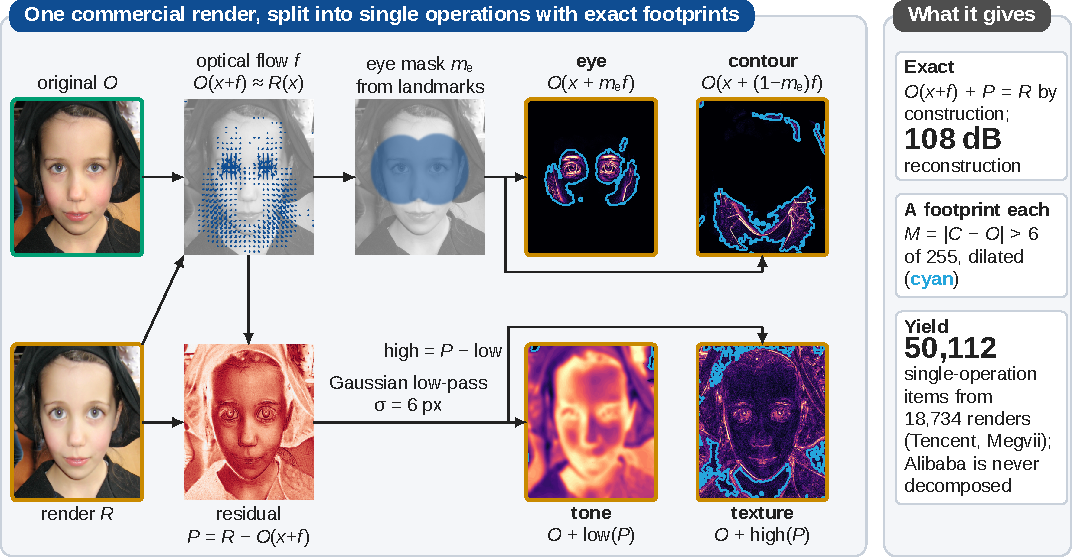
\includegraphics[width=\textwidth]{figs/fig_engine.pdf}
\caption{Splitting a commercial render into single operations (Tencent, FFHQ 60002; this render applies whitening,
smoothing, face lifting and eye enlarging at once). Top: the optical flow $f$, drawn as arrows six times their length every
16 pixels, is split by the eye mask into the eye and contour warps. Bottom: the residual $P$ (red brighter, blue darker) is
split by a Gaussian low-pass into tone and texture. Component tiles show $|C-O|$, each scaled to its own 99.5th percentile,
with the exact footprint $M$ outlined in cyan. The four components computed for this figure are bit-identical to those of
the training data.}
\label{fig:engine}
\end{figure*}

\subsection{Training recipe}
\label{sec:recipe}

The detector is a frozen CLIP ViT-L/14~\cite{clip} with rank-16 LoRA~\cite{lora} on the query, key, value and output
projections of all 24 blocks, 3.16 M of 306 M parameters trained (Figure~\ref{fig:model}). Each training step draws one
genuine, one forged and one beautified item from one genuine frame. The pool holds 41,512 genuine FF++ (c23) frames and
7,015 FFHQ originals; 41,526 FF++ forgeries, 61,510 part-level edits with exact footprints, and self-blends built online;
and, for the beautified class, 18,734 renders of two commercial retouching services (Tencent and Megvii), their 50,112
single-operation components (Section~\ref{sec:engine}), scripted operations, colour filters and colour grading. The forged
item is beautified on top about half of the time, so smoothing is seen on both classes.

One linear head on the pooled CLS token gives a forged logit $f$ and a beautified logit $b$, combined as
$P(\text{forged})=\sigma(f)$, $P(\text{beautified})=(1-\sigma(f))\,\sigma(b)$ and $P(\text{real})=(1-\sigma(f))(1-\sigma(b))$,
so the forgery decision reads $f$ only. A second head scores the four operations, trained wherever the operation is known.
A third regresses how much each was applied (the measured change in eye width, jaw width, skin lightness and
high-frequency energy) with an L1 loss; it is auxiliary, and its outputs are not shown on the page because they failed their
pre-declared check (Spearman correlation 0.31 at best on Alibaba, against a bar of 0.6). A step takes 16 genuine frames with their items, 48 images; AdamW at
$10^{-4}$ with cosine decay, 8 epochs, and the checkpoint is chosen on validation data only. The Alibaba service is never used
in training. Two seeds are reported throughout.

\begin{figure*}[t]
\centering
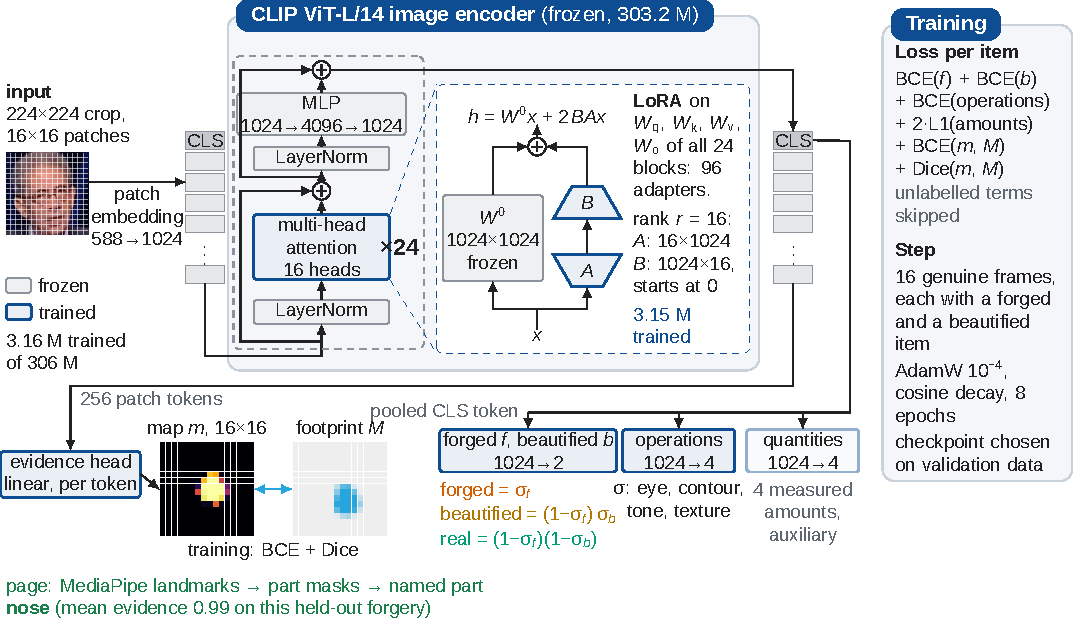
\includegraphics[width=\textwidth]{figs/fig_model.pdf}
\caption{The model (main checkpoint, seed 1), drawn from the training code. Top: the frozen CLIP ViT-L/14 image encoder;
one of its 24 Transformer blocks is shown, and the LoRA adapter added to each of its four attention projections is enlarged
($B$ starts at zero, so training starts from CLIP). Bottom: the heads. One linear head on the pooled CLS token gives the
forged and beautified logits ($\sigma_f=\sigma(f)$); the forgery score never reads $b$. The evidence head is applied to each
of the 256 patch tokens and gives the $16\times16$ map $m$, trained against the exact footprint $M$ at the same grid; both are
shown for the held-out part-level forgery of Figure~\ref{fig:method} (FF++ test frame 682, nose from a donor). Blue: trained;
grey: frozen.}
\label{fig:model}
\end{figure*}

\subsection{Evidence head and part naming}
\label{sec:evidence}

\begin{figure*}[t]
\centering
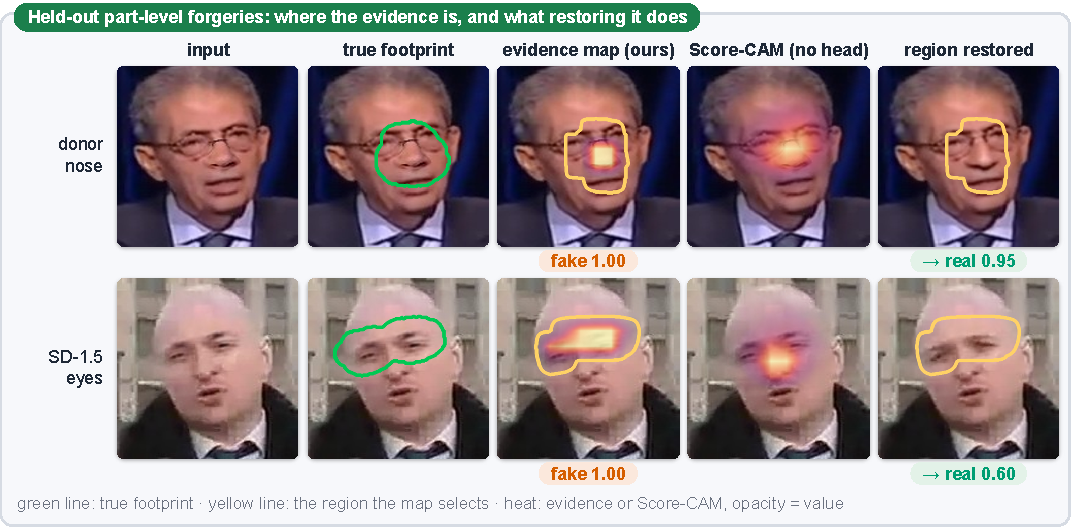
\includegraphics[width=\textwidth]{figs/fig_evidence.pdf}
\caption{Held-out part-level forgeries: input, true footprint, our evidence map with the decision, Score-CAM on the same
backbone without the head, and the result of restoring the marked region.}
\label{fig:evidence}
\end{figure*}

A linear map from the 256 patch tokens gives a $16\times16$ evidence map, trained against the exact footprint of each edit
(binary cross-entropy plus Dice). The classifier does not read the map, so whether the map explains the decision has to be
tested. MediaPipe's 478 landmarks give masks for eyes, nose, mouth, skin and contour; the part with the highest mean evidence
is named, and the whole face is named when eyes, nose and mouth all reach 0.5.

\emph{Restoration test.} For a detected part-level forgery with footprint $M$, let $\hat A$ be the $|M|$ highest cells of the
map. Restoring $\hat A$ to the original pixels and asking the model again shows whether the region is sufficient for its
decision; restoring everything except $\hat A$ shows whether it is necessary. The ceiling is the same test with the true
footprint.

\subsection{Sentences composed and checked by code}
\label{sec:sentences}

The decision, the three probabilities, the operation scores, the mean evidence per part and the named part form one
record. Code composes the explanation from the record: the decision with its score, the region, the smoothing score and whether
it reaches the threshold (the other three operations are not named, because they are unreliable across services), and a fixed sentence that the score is the model's raw output and not a calibrated probability.
Before display a rule checker matches the text to the record on decision, region, operations, numbers, forbidden phrases and
sentence count (rules H1 to H6), and rejects a decision score compared with the operation threshold (G7), any wording about
certainty, negated forms included (G8), and a decision score attached to a face part (G9). Four questions the record cannot
answer (the difference from an original, identity, certainty, the meaning of the score) get fixed sentences.
Figure~\ref{fig:explain} shows the composition and the checks on one held-out record.

\begin{figure*}[t]
\centering
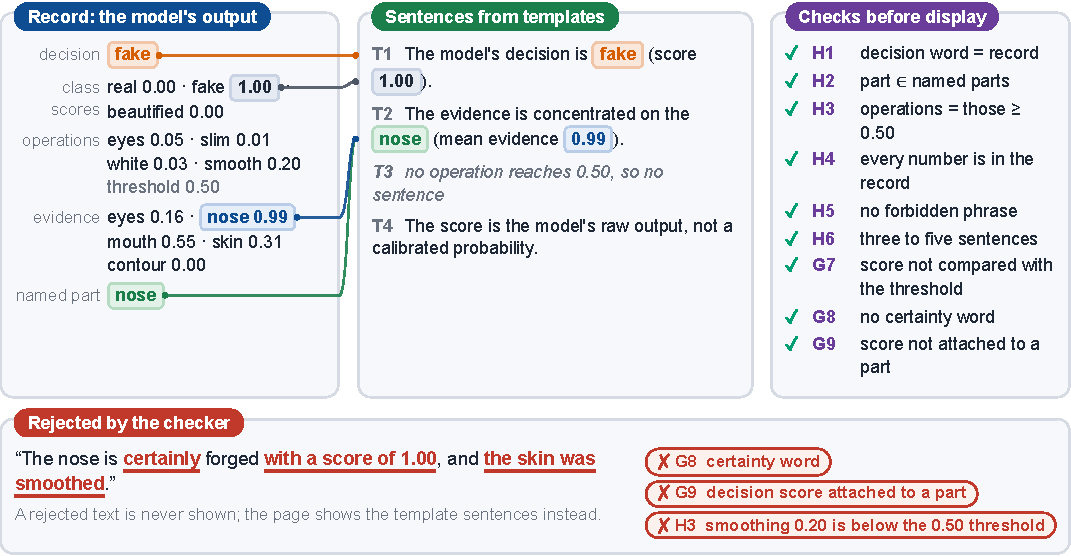
\includegraphics[width=\textwidth]{figs/fig_explain.pdf}
\caption{How the sentences are composed and checked, on one held-out record (FFHQ 17042 with the nose replaced from
another photograph). Each line traces a value in the sentences back to the record; the third template stays silent
because no operation reaches the threshold. The bottom row is a sentence the checker rejects, with the rule each
underlined phrase breaks.}
\label{fig:explain}
\end{figure*}

% ------------------------------------------------------------------ 5
\section{System Implementation and Experiments}

\subsection{The browser system}
\label{sec:system}

The page is the product: a visitor chooses or takes a face photograph, and the page answers real, forged or beautified,
outlines the evidence on the face, names the part, shows the checked sentences and, for a beautified verdict, the four
operation scores. Figure~\ref{fig:output} shows the result card on a bundled example, a held-out part-level forgery. The page loads MediaPipe's face landmarker and an ONNX
model, crops the face exactly as in training, runs the model with ONNX Runtime Web on WebAssembly, and computes the contour,
the part name and the sentences on the device. No server is involved and nothing is uploaded. The page also ships a set of
cases with known answers drawn by a fixed seed, so that a visitor can see the system's errors as well as its successes.
Table~\ref{tab:models} lists every model that appears in this report.

\begin{table}[!htb]
\centering
\caption{The models in this report. The previous browser model is kept on disk for rollback and is not offered on the page.}
\label{tab:models}
\footnotesize
\setlength{\tabcolsep}{3pt}
\begin{tabularx}{\columnwidth}{@{}>{\raggedright\arraybackslash}p{2.0cm}>{\raggedright\arraybackslash}p{2.75cm}>{\raggedright\arraybackslash}X@{}}
\toprule
Model & Backbone, parameters & Role \\
\midrule
Main (seeds 1, 2) & CLIP ViT-L/14 + LoRA; 3.2 M trained of 306 M & every number of Sections~\ref{sec:res-threeclass}--\ref{sec:res-text}; GPU only \\
Browser, shipped & EfficientNet-B4, same heads; 17.6 M, 67 MB & the page's default; gate in Table~\ref{tab:browser} \\
Browser, small & RepViT, same heads; 4.7 M, 19 MB & option for older phones; balanced accuracy 66.2\% \\
17 published detectors & released weights & the audit only (Section~\ref{sec:res-audit}) \\
\bottomrule
\end{tabularx}
\end{table}

\begin{figure*}[t]
\centering
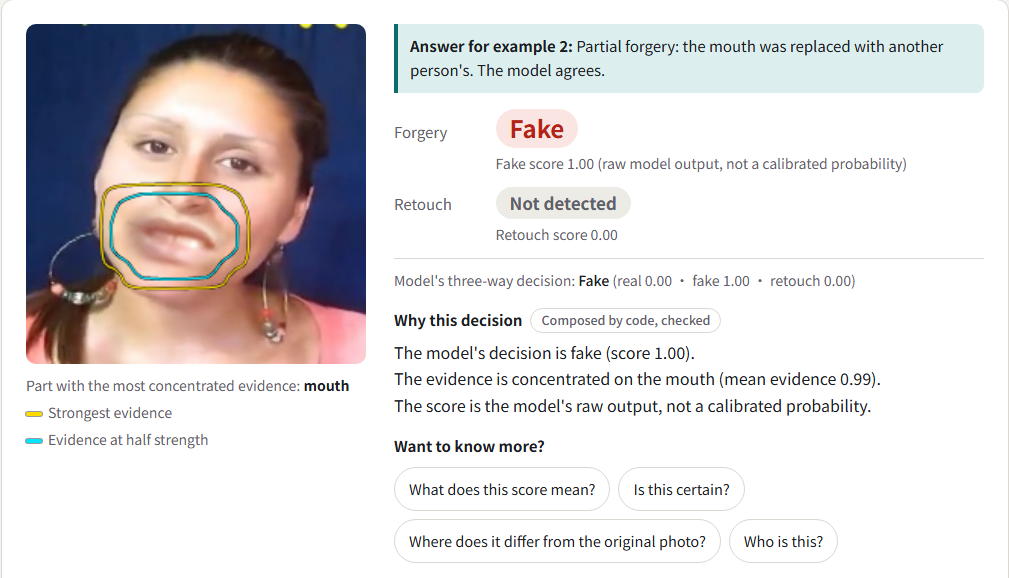
\includegraphics[width=0.86\textwidth]{figs/fig_output_a_crop.png}
\caption{The page's result card on a bundled example: a held-out part-level forgery, an FF++ test frame whose mouth was
replaced with that of another test-video subject (shipped browser model, 1366 px viewport). Left: the photo with the evidence
outlines (yellow: the 12\% of the map with the strongest evidence; cyan: evidence score at least 0.5) and the named part,
here the mouth. Right: the forgery and retouch chips with raw scores, the three-way decision, the sentences composed by code
with the badge of the checker, and the follow-up questions. The example was chosen to show the outlines; the restoration
test (Table~\ref{tab:restore}) measures the map on every held-out forgery. Every sentence passes the page's own rule checker
before it is shown (Section~\ref{sec:sentences}).}
\label{fig:output}
\end{figure*}

The CLIP model (306 M parameters) is too large for a browser, so the page runs an EfficientNet-B4~\cite{efficientnet} with the
same heads and evidence map (17.6 M parameters, 67 MB). An earlier browser model trained with an older recipe, which showed
beautified views to genuine faces only, let beautified deepfakes through as often as the worst published detector (miss rise
+23.9 points on Celeb-DF-B), the very trap Figure~\ref{fig:exposure} predicts. The shipped model is trained with the recipe of
Section~\ref{sec:recipe} plus 22,135 FairFace training photographs as additional genuine bases, so that ordinary photographs
are not out of distribution. Its acceptance gate was written before training; it passed four of five items and failed the
escape item (Section~\ref{sec:res-browser}).

\subsection{Experimental setup}

Development and test data are separated by video, FFHQ index and file. The explanation rules were developed on a 429-image
set and evaluated on a 361-image holdout (100 FF++ genuine, 40 FF++ forged, 72 Alibaba renders, 99 part-level forgeries, 50
scripted FFHQ edits). Part-level forgeries for the restoration test are built from FF++ test frames with test-video donors by
three editors, one of which (SDXL inpainting) was never used in training. Checkpoints are selected on validation data only.
Alibaba renders and Celeb-DF-B were never used for training or selection, but they were read repeatedly during the study, so
they are analysis sets rather than blind tests.

% ------------------------------------------------------------------ 6
\section{Performance Evaluation and Results}

\subsection{Three-class accuracy on held-out data}
\label{sec:res-threeclass}

Table~\ref{tab:threeclass} gives the per-class recall on the FF++ (c23) test split, 7,936 frames of 140 videos never used
for training or selection, and the direction of the errors. The main model keeps every class above 80\% on seed 1; its errors
are genuine frames called beautified (11.4\%) rather than forged (5.9\%), and beautified frames called genuine (9.0\%) rather
than forged (4.3\%). The shipped browser model is within about 5 points of it on every class. On ordinary photographs outside
FF++ the main model calls 78.4\% of the 2,210 untouched FFHQ originals real, 20.8\% beautified and 0.8\% forged; the
cross-dataset video results are in Table~\ref{tab:browser}.

\begin{table}[!htb]
\centering
\caption{Three-class recall and the direction of the errors (\%) on the FF++ (c23) test split. Main: CLIP ViT-L/14 + LoRA,
seeds 1 and 2. Browser: EfficientNet-B4; shipped = the model on the page since 2026-10-30, previous = the model it replaced
(Section~\ref{sec:res-browser}). Best of each row in bold.}
\label{tab:threeclass}
\footnotesize
\setlength{\tabcolsep}{4pt}
\begin{tabular}{@{}lcccc@{}}
\toprule
 & \multicolumn{2}{c}{Main} & \multicolumn{2}{c}{Browser} \\
\cmidrule(lr){2-3}\cmidrule(lr){4-5}
 & s1 & s2 & shipped & previous \\
\midrule
recall, real & \textbf{82.7} & 76.9 & 81.7 & 74.2 \\
recall, forged & 90.9 & 92.3 & 91.6 & \textbf{93.3} \\
recall, beautified & \textbf{86.7} & 86.3 & 81.2 & 76.4 \\
\midrule
real $\to$ forged & \textbf{5.9} & 9.0 & 7.2 & 11.6 \\
real $\to$ beautified & 11.4 & 14.1 & \textbf{11.1} & 14.1 \\
beautified $\to$ forged & \textbf{4.3} & 6.5 & 7.1 & 11.7 \\
beautified $\to$ real & 9.0 & \textbf{7.3} & 11.8 & 11.9 \\
\bottomrule
\end{tabular}
\end{table}

\subsection{The audit: seventeen detectors, two directions}
\label{sec:res-audit}

Table~\ref{tab:audit} gives the audit. Sixteen of seventeen detectors score the smoothed face above its own original in most
pairs, fifteen in 89 to 99\% of pairs; NPR, whose scores saturate at 1.0 on these stills, does not. At its own threshold,
thirteen of seventeen call 36 to 69\% of the smoothed genuine faces fake. The effect is specific to smoothing: the same
service's whitening, face slimming and eye enlarging are accused at about the nominal 5\%. On video, app beautification
raises the miss rate of 14 of the 17 detectors by 3 to 22 points beyond re-encoding. An open-source beauty engine (GPUPixel)
reproduces the accusation: at its strongest skin smoothing 14 of 15 face detectors accuse more than 15\% of genuine
Celeb-DF-v2 frames, while our model accuses 13.7 / 13.1\% and keeps an AUC of 0.80 / 0.82.

\begin{table}[!htb]
\centering
\caption{The audit. Accusation: on 2,210 commercial Smoothing-90 pairs, the share of pairs whose render scores above its own
original, and the renders accused at the threshold that accuses 5\% of the originals (\%). Escape: on Celeb-DF-B app presets,
video AUC after beautification and the miss rise net of re-encoding (points). Bold: best, underlined: second (above-original
closest to 50, accused lowest, AUC highest, miss rise closest to 0; NPR, saturated, not ranked). FF++ only: the published
detectors' training videos (--: no retouching data); the other rows of ours used more data, a reference, not a ranking.}
\label{tab:audit}
\footnotesize
\renewcommand{\arraystretch}{0.92}
\begin{adjustbox}{max width=\columnwidth}
\begin{tabular}{@{}lcccc@{}}
\toprule
 & \multicolumn{2}{c}{Accusation} & \multicolumn{2}{c}{Escape} \\
\cmidrule(lr){2-3}\cmidrule(lr){4-5}
Detector & above orig. & at 5\% FPR & AUC & miss rise \\
\midrule
Xception & 95.2 & 51.6 & 0.737 & +10.9 \\
EfficientNet-B4 & 93.7 & 36.3 & 0.762 & \underline{+3.4} \\
F3Net & 97.8 & 50.6 & 0.731 & +10.9 \\
SPSL & 97.3 & 51.2 & 0.727 & +12.4 \\
UCF & 95.4 & 41.4 & 0.777 & +11.3 \\
RECCE & 96.5 & 36.8 & 0.723 & +13.8 \\
CORE & 96.6 & 54.8 & 0.752 & +13.5 \\
SRM & 99.3 & 62.8 & 0.733 & +15.3 \\
SBI~\cite{sbi} & 96.2 & 37.3 & 0.752 & +21.8 \\
CADDM~\cite{caddm} & \underline{60.9} & \textbf{6.3} & 0.762 & \textbf{$-$2.9} \\
LAA-Net~\cite{laanet} & 89.2 & 17.2 & 0.698 & +14.7 \\
UnivFD~\cite{univfd} & 90.4 & 16.6 & 0.624 & $-7.2$ \\
NPR~\cite{npr} & 31.8 (sat.) & 0.0 & 0.498 & $-0.7$ \\
Effort~\cite{effort} & 95.6 & 43.2 & 0.807 & +11.0 \\
Forensics Ad.~\cite{forensicsadapter} & 93.3 & 39.7 & 0.828 & +15.2 \\
GenD~\cite{gend2026} & 98.5 & 68.7 & 0.807 & +12.0 \\
DFD-HR~\cite{dfdhr2026} & 99.0 & 64.9 & 0.838 & +3.6 \\
\midrule
Ours, FF++ only, s1 & -- & -- & 0.872 & +7.5 \\
\phantom{Ours, FF++ only,} s2 & -- & -- & 0.870 & +9.1 \\
Ours, three-way, s1 & 32.5 & 8.6 & 0.866 & +6.7 \\
\phantom{Ours, three-way,} s2 & \textbf{41.3} & 12.5 & 0.883 & +8.3 \\
Ours, forgery head, s1 & 70.5 & 9.1 & \underline{0.896} & +7.0 \\
\phantom{Ours, forgery head,} s2 & 68.2 & \underline{6.5} & \textbf{0.904} & +5.7 \\
\bottomrule
\end{tabular}
\end{adjustbox}
\end{table}

No published detector is lower than ours in both directions of Table~\ref{tab:audit}. CADDM sits near the same corner on the raw
axes but accuses 13.8\% of beautified genuine frames, and its AUC after beautification is 0.10 lower. The forgery-head-only
row shows that neither property comes from the third class: it is as low on the accusation and higher in AUC.
Trained only on the FF++ videos of Effort, Forensics Adapter, GenD and DFD-HR, the recipe keeps 0.872 / 0.870 AUC after
beautification, above every published detector (paired intervals against Effort, Forensics Adapter and SBI exclude zero).

\subsection{Per operation and per strength}
\label{sec:res-perop}

Figure~\ref{fig:perop} breaks the accusation down by operation and strength. For eye enlarging, face slimming and whitening
every detector stays near the 5\% floor at every strength (Effort and UnivFD reach 11 to 17\% on the strongest eye
enlarging); for skin smoothing the published detectors rise with strength to 37 to 52\% at level 90 (UnivFD 16.6\%), while
ours stays between 5.0 and 12.5\%. On the same pairs our three-way decision calls a render forged in at most 0.8\% of
pairs at any operation and strength; smoothing is called beautified in 90 to 99\%
of pairs; eye enlarging, face slimming and whitening are called beautified in 46 to 72\% of pairs and otherwise real, although
the render's beautified score exceeds its own original's in 84 to 98\% of pairs. The three single operations are therefore
detected relative to the original but not reliably in absolute terms, the limitation stated in Section~\ref{sec:res-text}.

\begin{figure}[!htb]
\centering
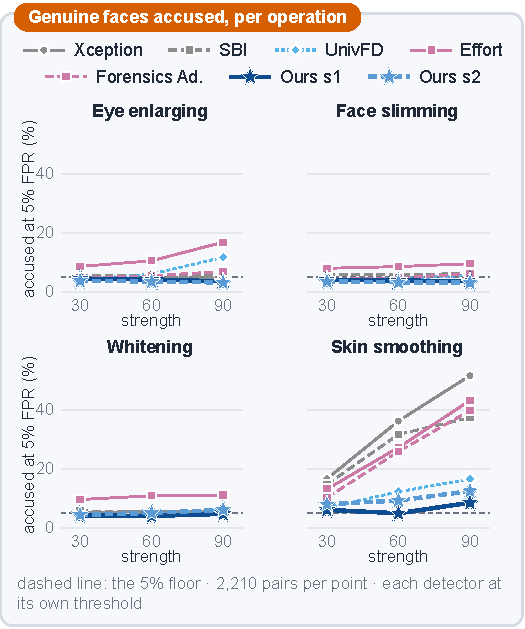
\includegraphics[width=\columnwidth]{figs/fig_perop.pdf}
\caption{Genuine faces accused after each retouching operation of the Alibaba service, at strengths 30, 60 and 90, at the
threshold that accuses 5\% of the untouched originals (dashed line). 2,210 pairs per cell. Five published detectors and
both seeds of our model.}
\label{fig:perop}
\end{figure}

\subsection{The cause and the mechanism}
\label{sec:res-cause}

\begin{figure}[!htb]
\centering
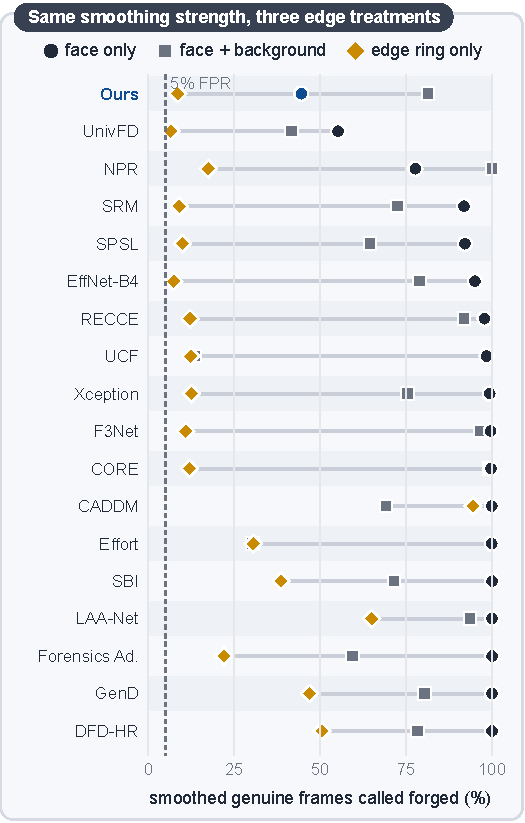
\includegraphics[width=\columnwidth]{figs/fig_context.pdf}
\caption{Same smoothing strength, three edge treatments: genuine Celeb-DF-v2 frames called forged at each detector's 5\%
threshold when only the face, the whole crop, or only a ring at the face edge is smoothed.}
\label{fig:context}
\end{figure}

Table~\ref{tab:exposure} gives the training arms. The accusation is what FF++ training gives by default: with no beautified
view, 43.5 to 56.1\% of the smoothed renders are accused, and showing smoothing to forged faces only raises it to 63.8\%.
Removing smoothing from otherwise rich beautified views leaves it at 55.3 and 67.1\%, so no other view substitutes for it.
Smoothing shown to genuine faces only brings the accusation to about 1\% and creates the opposite error, a miss rise of 56 to
63 points on smoothed forgeries. Shown to both classes it lowers the accusation to 6.9 to 11.7\%. With architecture, data and
recipe fixed, the answer to ``what decides the accusation'' is which class saw smoothing.

\begin{table}[!tb]
\centering
\caption{FF++-only arms of one model, one value per seed. Arm: which class saw beautified views in training; P1 smooth.: only
smoothing, on genuine faces; P2 w/o smooth.: both classes, smoothing removed; P2 same forms: both classes, the same smoothing
forms. Accused: commercial Smoothing-90 renders above the 5\% FPR threshold of their originals (\%). Miss rise: strongly
smoothed Celeb-DF-v2 forgeries (points; negative means smoothed faces of both classes are accused). AUC: Celeb-DF-v2 video.}
\label{tab:exposure}
\footnotesize
\setlength{\tabcolsep}{3pt}
\begin{adjustbox}{max width=\columnwidth}
\begin{tabular}{@{}llll@{}}
\toprule
Arm & accused & miss rise & AUC \\
\midrule
P0 none & 54.2/56.1/43.5 & $-$16.0/$-$11.8/+4.3 & .938/.938/.940 \\
P3 forged only & 63.8 & $-$38.5 & -- \\
P1 genuine only & 3.7/7.1/4.6 & +51.2 & .900/.910/.923 \\
P1 smooth. & 0.7/1.0/0.9 & +56.4/+60.0/+62.9 & .922/.929/.939 \\
P2 both & 11.7/7.1/6.9 & $-$26.5/$-$13.3 & .917/.920/.935 \\
P2 w/o smooth. & 55.3/67.1 & $-$28.9/$-$33.1 & .913/.924 \\
P2 same forms & 5.9/6.1 & +14.6/+17.5 & .919/.934 \\
\bottomrule
\end{tabular}
\end{adjustbox}
\end{table}

What do the detectors react to? With the bilateral strength held fixed, smoothing only a ring at the face-hull edge is accused
by a median of about 12\% against 92 to 100\% for the full face-local form, for 13 of 15 face detectors, and smoothing the
whole crop, face and background alike, is accused much less by the CLIP detectors (Figure~\ref{fig:context}). The accused
pattern is therefore a face smoother than its own context, which is the face-versus-context inconsistency that face-swap
detectors are built to find and that face-local beautification reproduces by construction. The reading has partial support
only: four detectors are accused on the whole crop as well, and our own model runs the other way.


Four repairs that leave training alone were measured, and each moves the error instead of removing it. Re-setting the
threshold on smoothed genuine faces leaves the published detectors missing 67 to 100\% of smoothed forgeries, because the scores
of the two classes coincide once both are smoothed. Routing smoothed inputs to an expert trained on smoothed copies clears the
accusation and raises the miss rate by 30 to 46 points. A smoothing-consistency loss is equivalent to moving the threshold. A
test-time rule that also scores a whole-crop-smoothed copy clears the accusation but is no better than the re-set threshold at
matched false alarms for any of 15 detectors. This is why the answer is a training recipe.

\subsection{Is the marked region the reason?}
\label{sec:res-evidence}

Table~\ref{tab:restore} and Figure~\ref{fig:evidence} give the restoration test on held-out part-level forgeries. Restoring the
region the evidence head marks removes 93.5 to 94.0\% of the detections, within 0.1 points of restoring the true footprint,
and restoring everything else removes at most 0.4\%: the region is sufficient and necessary for the model's own decision.
Heat maps on the same backbone remove 45 to 57\%, not far above a fixed region in the centre of the face. Repeated on the
named part rather than the map, on the 82 correctly detected part-level forgeries of the holdout, restoring the named part
removes 85.4\% of detections against 87.8\% for the map and 13.9\% for a random other part. For whole-face swaps no method
finds a small sufficient region, and the text then says that the evidence is spread over the whole face.

\begin{table}[!htb]
\centering
\caption{Restoration test on held-out part-level forgeries; each cell gives donor transplant / SD-1.5 inpainting / SDXL
inpainting, the last never seen in training. IoU with the true footprint, and the share of detections that leave ``fake''
when the marked region is restored (region) or when everything else is (rest), in \%.}
\label{tab:restore}
\footnotesize
\setlength{\tabcolsep}{3pt}
\begin{adjustbox}{max width=\columnwidth}
\begin{tabular}{@{}llll@{}}
\toprule
Map & IoU & flip, region & flip, rest \\
\midrule
Centre prior & .31/.25/.26 & 38.6/40.9/40.2 & 17.0/17.9/17.7 \\
Grad-CAM~\cite{gradcam} & .37/.26/.27 & 50.9/45.4/48.0 & 15.2/25.0/23.6 \\
Grad-CAM++~\cite{gradcampp} & .41/.33/.33 & 51.7/47.8/48.8 & 7.2/16.7/19.1 \\
Score-CAM~\cite{scorecam} & \underline{.41/.33/.34} & \underline{56.5/52.4/52.4} & \underline{5.9}/15.4/17.1 \\
Ours, evidence head & \textbf{.83/.84/.83} & \textbf{94.0/93.6/93.5} & \textbf{0.1/0.4/0.3} \\
\midrule
True footprint (ceiling) & 1 & 94.1/93.7/93.6 & -- \\
\bottomrule
\end{tabular}
\end{adjustbox}
\end{table}


\subsection{Sentences and free-form descriptions}
\label{sec:res-text}

On all 361 holdout records the composed sentences pass the six rules, as they must by construction, since composer and checker
read the same record. The checker earned its place on a path that was removed: a language model (Qwen2.5-7B) that only reworded
the facts passed the six rules and still wrote sentences the record did not support, such as a decision score ``concentrated
on the mouth''. Two rules added afterwards (G8, G9) blocked 390 English and 206 Chinese texts that had been shipped. Once every
number was moved into code, the model's wording shrank to about 20 distinct strings per style and differed from the template
in nothing that was measured, so the shipped system has no language model.

Free-form descriptions fail a more basic test (Table~\ref{tab:vlm}). A judge model sees an edited face and two sentences, one
written for it and one for its untouched original, and picks the matching one; an image-specific writer should be well above
50\%, and a positive control with two different people is matched at 95 to 99\%. No writer is above chance. Fine-tuning raised
BLEU-4 from 6.8 to 38.9, yet one fixed sentence per part scores higher on both text metrics with no image information, so text
similarity cannot tell a describer from a constant. A model sentence would also raise the time per image from 0.04~s to about
1~s and GPU memory from 1.2~GB to 17.8~GB.

\begin{table}[!htb]
\centering
\caption{Blind matching of free-form descriptions (edited face against its own original; matching with its 95\% interval;
identical: share of identical sentences).}
\label{tab:vlm}
\footnotesize
\begin{adjustbox}{max width=\columnwidth}
\begin{tabular}{@{}lccc@{}}
\toprule
Writer & matching (\%) & identical & BLEU-4 / CIDEr \\
\midrule
Qwen2.5-VL-7B & 52.8 [49.4, 56.2] & 36.4\% & 6.8 / 0.19 \\
\quad + LoRA, 20k sentences & 51.3 [49.3, 53.2] & 74.5\% & 38.9 / 4.20 \\
FakeVLM~\cite{fakevlm2025} & 50.8 [48.3, 53.2] & 37.3\% & -- \\
Constant sentence per part & n/a & -- & 44.4 / 4.32 \\
\bottomrule
\end{tabular}
\end{adjustbox}
\end{table}

\subsection{The browser model}
\label{sec:res-browser}

The browser model had to pass a gate written before training. Table~\ref{tab:browser} compares it with the earlier browser
model and the CLIP model.

\begin{table}[!htb]
\centering
\caption{Browser models against the gate written before training. Miss rise: beautified Celeb-DF-B deepfakes, points
(previous +23.9 [20.2, 27.7], shipped +19.1 [16.2, 22.1]); FairFace: ordinary photographs called real; S-90: commercial
Smoothing-90 renders; restoration: detections removed by restoring the named region on held-out part-level forgeries; all
other rows in \%.}
\label{tab:browser}
\footnotesize
\setlength{\tabcolsep}{3pt}
\begin{tabular}{@{}lcccc@{}}
\toprule
 & gate & previous & shipped & CLIP (s1) \\
\midrule
Celeb-DF-B miss rise & $\le 11.0$ & +23.9 & \textbf{+19.1} (fail) & +6.7 \\
FairFace called real & $\ge 70$ & 29.2 & 95.7 & 23.2 \\
S-90 called fake & $\le 2$ & 0.4 & 1.0 & 0.8 \\
S-90 accused at 5\% FPR & $\le 15$ & 6.3 & 7.3 & 8.6 \\
Celeb-DF-v2 frame AUC & $\ge 0.8275$ & 0.848 & 0.849 & 0.891 \\
DFD frame AUC & $\ge 0.8952$ & 0.915 & 0.917 & 0.956 \\
FF++ beautified$\to$forged & $\le 13.7$ & 11.7 & 7.1 & 4.3 \\
Restoration & $\ge 80$ & 87.4 & 91.5 & 94.0 \\
\bottomrule
\end{tabular}
\end{table}

The shipped model (epoch 11 of 12, chosen on validation data only) passes four of the five items and fails the escape item:
beautified Celeb-DF-B deepfakes raise its miss rate by 19.1 points against a bar of 11.0. It is lower than the previous
browser model's 23.9, but the two intervals overlap, so the improvement is not shown. The pre-declared rule was to keep the
previous model on a failure; we shipped the new one by decision, because it is no worse on any item and the previous model
called only 29.2\% of ordinary FairFace photographs real (35.8\% forged), against 95.7\% for the new one. The small
backbone does not inherit the CLIP model's low escape (+19.1 against +6.7), which is the main remaining limitation of the
page. The ONNX export agrees with the PyTorch model on 50 of 50 decisions and named parts.
On one WebAssembly thread a photograph takes a median 0.51~s on a desktop and 0.59~s in Safari on an iPhone (40 timed runs
on the four bundled examples); the 67~MB model downloads once per visit, in 52~s on the phone's connection. The small RepViT
model of Table~\ref{tab:models} takes 0.15 and 0.19~s; it is faster and weaker.

\subsection{Costs}
\label{sec:costs}

Four costs are real and the page shows them next to the answer. \emph{Reenactment}: the three-way model is near chance on DF40
reenactment in the Celeb-DF domain (AUC 0.50 / 0.56). \emph{Untouched faces called beautified}: 20.8 / 19.6\% of the retouching
service's originals. \emph{The beautified class as a hiding place}: beautification moves 10.9 / 9.8 points of Celeb-DF-B
deepfakes into ``beautified'' beyond re-encoding, so the page shows the forgery score next to every ``beautified'' verdict.
\emph{Only smoothing can be named}: within one service, a classifier trained on one operation separates renders from
originals at AUROC 0.93 (eye enlarging) to 0.9995 (smoothing), but trained on the two other services and tested on Alibaba
the first three operations fall to 0.69--0.72 while smoothing stays at 0.999, so the sentences name smoothing only.

% ------------------------------------------------------------------ 6b
\section{Team Collaboration}

The three members shared one repository and one experiment log. Every experiment was registered before it ran, with its
data, its pass or fail threshold and the result file it would write, and the readout was entered the same day, whether it
passed or not, so the lines that failed are on record next to the one that succeeded.
Each line of work lives in its own folder with a timestamped log, and every number in this report is read from a result file
by a script, so a change in one place changes the table, the figure and the text together. Code written by one member was
run by another before its numbers were trusted. The report, the poster, the video and the browser page were split by
member and reviewed by the other two, and the weekly meeting with the laboratory decided which lines to continue.

% ------------------------------------------------------------------ 7
\section{Important Contributions}

\textbf{Research findings.} (1) Beautification breaks face-forgery detectors in both directions: sixteen of seventeen
published detectors score a smoothed genuine face above its own original, and app beautification lets deepfakes through
(Section~\ref{sec:res-audit}). (2) The cause is on the training side, not in the test images: in a controlled comparison that
changes only which class sees skin-smoothed views, showing smoothing to forged faces only produces the accusation, to genuine
faces only produces the escape, and to both produces neither (54\% to 12\% accused, Section~\ref{sec:res-cause}). (3) The
mechanism is a face smoother than its context, which the detectors read as a pasted face. (4) Free-form descriptions written by
vision-language models are matched to their own photograph as often as a coin flip (Section~\ref{sec:res-text}).

\textbf{Method.} A three-way detector (real, forged, beautified) trained from paired edits whose footprint is known exactly
(Figure~\ref{fig:method}): commercial renders split by optical flow and photometric residual into single operations,
part-level forgeries, and FF++ triplets in which both classes see smoothing. Factorised class logits make the forgery score
independent of the beautified logit. An evidence head trained against the footprints marks the edited region, and restoring
the original pixels inside the mark removes 94\% of the model's part-level forgery decisions, against about half for a
post-hoc heat map. Landmarks turn the map into a named part, and code composes and checks every sentence, so no language
model describes the image.

\textbf{Application.} The whole chain runs in a web browser, 0.59~s per photograph on an iPhone with nothing uploaded. The
page ships cases with known answers, shows the forgery score next to every ``beautified'' verdict, and its model passed four
of the five items of a gate written before training; the failed item is stated (Section~\ref{sec:res-browser}).
The detector, the audit and the training-exposure experiment are also reported in a paper of our laboratory written by the
same students.

% ------------------------------------------------------------------ 9
\section{Conclusion}

Face-forgery detectors call a skin-smoothed genuine face fake and let an app-beautified deepfake through, and which class saw
smoothing in training decides the direction. The system built here says real, forged or beautified, marks the part of the face
its decision rests on, and shows only sentences that code has checked, in a browser on the user's phone. Its costs are
stated beside the answer: beautified deepfakes can hide in the third class, some untouched photographs are called beautified,
and only smoothing can be named.

\bibliographystyle{IEEEtran}
\bibliography{refs}

\end{document}
